% Copyright (c) 2015 by the University of Waikato, Hamilton, NZ.
% This work is made available under the terms of the 
% Creative Commons Attribution-ShareAlike 3.0 license, 
% http://creativecommons.org/licenses/by-sa/3.0/. 
%
% Version: $Revision: 3363 $

\documentclass[a4paper]{book}

\usepackage{wrapfig}
\usepackage{graphicx}
\usepackage{hyperref}
\usepackage{multirow}
\usepackage{scalefnt}
\usepackage{tikz}
\usepackage{varwidth}

% watermark -- for draft stage
\usepackage[firstpage]{draftwatermark}
\SetWatermarkLightness{0.9}
\SetWatermarkScale{5}

% Copyright (c) 2009 by the University of Waikato, Hamilton, NZ. 
% This work is made available under the terms of the 
% Creative Commons Attribution-ShareAlike 4.0 license,
% http://creativecommons.org/licenses/by-sa/4.0/.
%
% Version: $Revision: 5479 $

\newenvironment{tight_itemize}{
\begin{itemize}
  \setlength{\itemsep}{1pt}
  \setlength{\parskip}{0pt}
  \setlength{\parsep}{0pt}}{\end{itemize}
}

\newenvironment{tight_enumerate}{
\begin{enumerate}
  \setlength{\itemsep}{1pt}
  \setlength{\parskip}{0pt}
  \setlength{\parsep}{0pt}}{\end{enumerate}
}

% if you just need a simple heading
% Usage:
%   \heading{the text of the heading}
\newcommand{\heading}[1]{
  \vspace{0.3cm} \noindent \textbf{#1} \newline
}

\newcommand{\icon}[1]{\tikz[baseline=-3pt]\node[inner sep=0pt,outer sep=0pt]{\includegraphics[height=1.1em]{#1}};}


\title{
  \textbf{ADAMS} \\
  {\Large \textbf{A}dvanced \textbf{D}ata mining \textbf{A}nd \textbf{M}achine
  learning \textbf{S}ystem} \\
  {\Large Module: adams-video} \\
  \vspace{1cm}
  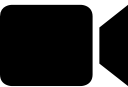
\includegraphics[width=2cm]{images/video-module.png} \\
}
\author{
  Peter Reutemann \\
  Steven Brown
}

\setcounter{secnumdepth}{3}
\setcounter{tocdepth}{3}

\begin{document}

\begin{titlepage}
\maketitle

\thispagestyle{empty}
\center
\begin{table}[b]
	\begin{tabular}{c l l}
		\parbox[c][2cm]{2cm}{\copyright 2015-2016} &
		\parbox[c][2cm]{5cm}{
\includegraphics[width=5cm]{images/coat_of_arms.pdf}} \\
	\end{tabular}
	
\includegraphics[width=12cm]{images/cc.png} \\
\end{table}

\end{titlepage}

\tableofcontents
\listoffigures
%\listoftables

%%%%%%%%%%%%%%%%%%%%%%%%%%%%%%%%%%%
\chapter{Flow}
The video module offers some actors for basic video display and processing support.

\noindent Available standalones:
\begin{tight_itemize}
    \item \textit{RecordingSetup} -- configures a recording setup (sound/screen/webcam).
    \item \textit{StartRecording} -- starts a defined recording setup.
    \item \textit{StopRecording} -- stops a defined recording setup.
\end{tight_itemize}

\noindent Available sources:
\begin{tight_itemize}
    \item \textit{ListWebcams} -- lists the names of all available webcams
    attached to the computer\footnote{adams-video-list\_webcams.flow}.
    \item \textit{WebcamImage} -- outputs images from the selected webcam
    attached to the computer\footnote{adams-video-webcam.flow}.
    \item \textit{WebcamInfo} -- outputs images from the selected webcam
    \footnote{adams-video-webcam\_info.flow}.
\end{tight_itemize}

\noindent Available transformers:
\begin{tight_itemize}
	\item \textit{AddTrailBackground} -- adds a image as trail
	background\footnote{adams-video-track\_objects-predefined3.flow}
	\item \textit{AddTrailStep} -- adds an additional step to the trail
	passing through\footnote{adams-video-track\_objects-predefined3.flow}.
	\item \textit{ExtractTrackedObject} -- extracts a tracked
	object in an image and forwards it as new image.
	container\footnote{adams-video-track\_objects-user\_selected\_object.flow}.
	\item \textit{GetTrailBackground} -- retrieves the trail background image, if any.
	\item \textit{MjpegImageSequence} -- generates an image sequence
	from MJPEG movies, one frame at a time\footnote{adams-video-play\_mjpeg\_video.flow}.
	\item \textit{MovieImageSequence} -- generates an image sequence
	from movies, one frame at a time (uses Xuggle\cite{xuggle}\footnote{adams-video-play\_mp4\_video.flow}).
	\item \textit{TrackObjects} -- tracks objects in images sequences,
	e.g., from movies\footnote{adams-video-track\_objects-predefined.flow, adams-video-track\_objects-predefined2.flow}.
	\item \textit{TrailFileReader} -- reads a trail from disk.
	\item \textit{TrailFileWriter} -- writes a trail to disk\footnote{adams-video-track\_objects-predefined3.flow}.
	\item \textit{TrailFilter} -- applies a filter to the trail passing through.
	\item \textit{TransformTrackedObject} -- transforms a tracked
	object in an image with a callable transformer, e.g., for blurring a
	face\footnote{adams-video-track\_objects-predefined2.flow}.
\end{tight_itemize}

\noindent Available sinks:
\begin{tight_itemize}
  \item \textit{AnimatedGifFileWriter} -- generates an animated GIF from
  an array of image files or images.
  \item \textit{FFmpeg} -- actor for processing videos using
  ffmpeg\cite{ffmpeg}\footnote{adams-video-ffmpeg.flow}.
  \item \textit{TrailDisplay} -- displays trail objects\footnote{adams-video-display\_trail.flow, adams-video-track\_objects-predefined3.flow}.
\end{tight_itemize}

\noindent Available conversions:
\begin{tight_itemize}
  \item \textit{QuadrilateralLocationCenter} -- outputs a Point2D object that
  is the center of the rectangle surrounding the quadrilateral coordinates.
  \item \textit{QuadrilateralLocationToString} -- turns the quadrilateral
  coordinates into a string.
  \item \textit{StringToQuadrilateralLocation} -- turns a string into quadrilateral
  locations.
\end{tight_itemize}

%%%%%%%%%%%%%%%%%%%%%%%%%%%%%%%%%%%
\chapter{Tools}

\section{Trail viewer}
The \textit{Trail viewer} is a simple tool for viewing trails of objects that
have been tracked using a flow. It can be used to apply filters to trails
and save those trails back to disk. Figure \ref{trail_viewer} shows a screenshot.

\begin{figure}[htb]
  \centering
  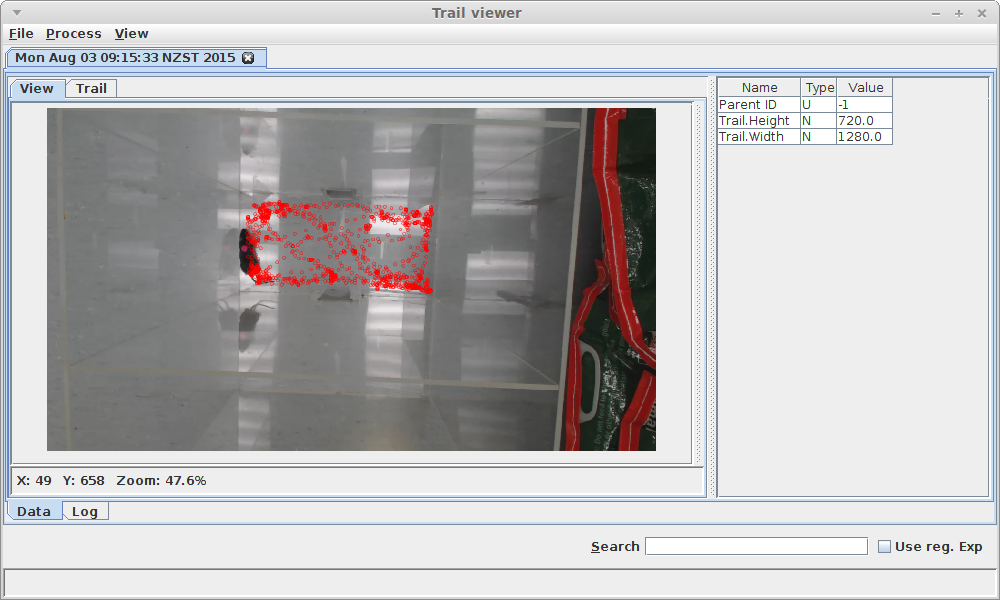
\includegraphics[width=12.0cm]{images/trail_viewer.png}
  \caption{Trail viewer displaying a mice trail overlayed on a background image.}
  \label{trail_viewer}
\end{figure}

%%%%%%%%%%%%%%%%%%%%%%%%%%%%%%%%%%%
\section{Annotator}

The annotator has three menus which we will cover in the following sections.

\subsection{Video Menu}
The video menu (see Figure \ref{AnnotatorVideoMenu}) lets you open video
files or quit the program. It also provides a list of recently opened videos.

\begin{figure}[htb]
  \centering
  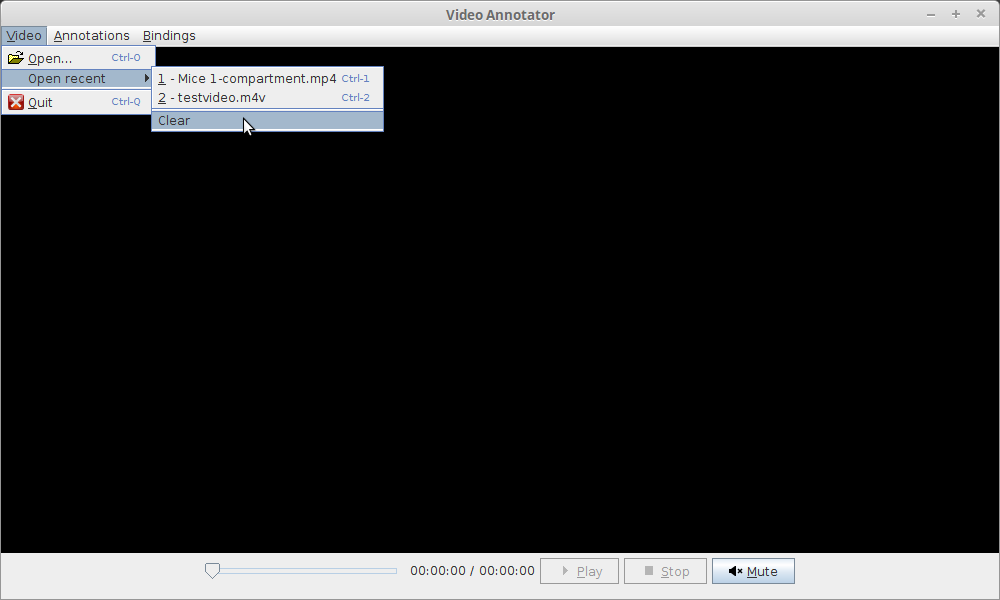
\includegraphics[width=12.0cm]{images/AnnotatorVideoMenu.png}
  \caption{Video menu.}
  \label{AnnotatorVideoMenu}
\end{figure}

\subsection{Annotations Menu}
This menu lets you create a new set of annotations or export the current
set to a spreadsheet file, e.g., CSV or, depending on modules present,
MS Excel (see Figure \ref{AnnotatorAnnotationMenu}).

\begin{figure}[htb]
  \centering
  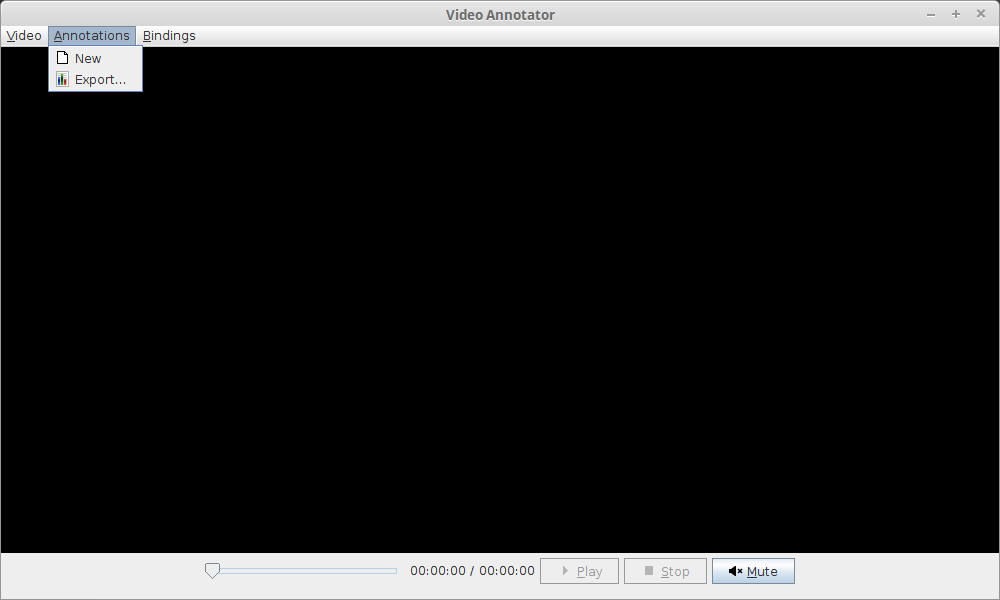
\includegraphics[width=12.0cm]{images/AnnotatorAnnotationMenu.png}
  \caption{Annotations menu.}
  \label{AnnotatorAnnotationMenu}
\end{figure}

\subsection{Bindings menu}
The bindings menu, as depicted in Figure \ref{AnnotatorBindingsMenu}, allows
for the creation of a new set of bindings, loading or saving bindings, and
editing the current bindings.

\begin{figure}[htb]
  \centering
  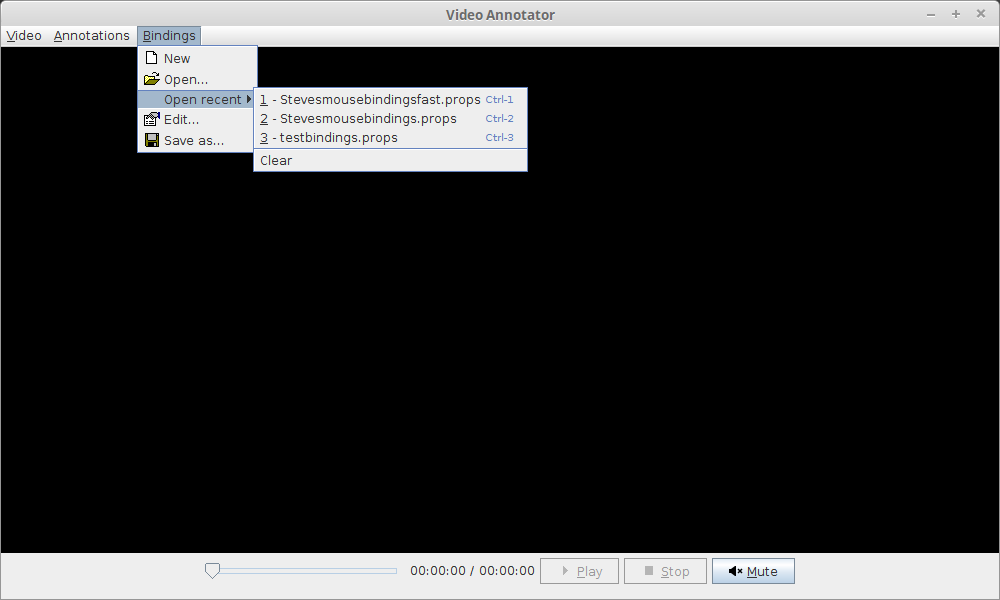
\includegraphics[width=12.0cm]{images/AnnotatorBindingsMenu.png}
  \caption{Bindings menu.}
  \label{AnnotatorBindingsMenu}
\end{figure}

\subsubsection{Edit Bindings}
When editing bindings you can add new bindings, edit a current binding or
remove selected bindings (see Figure \ref{AnnotationEditBindingsDialog}).

\begin{figure}[htb]
  \centering
  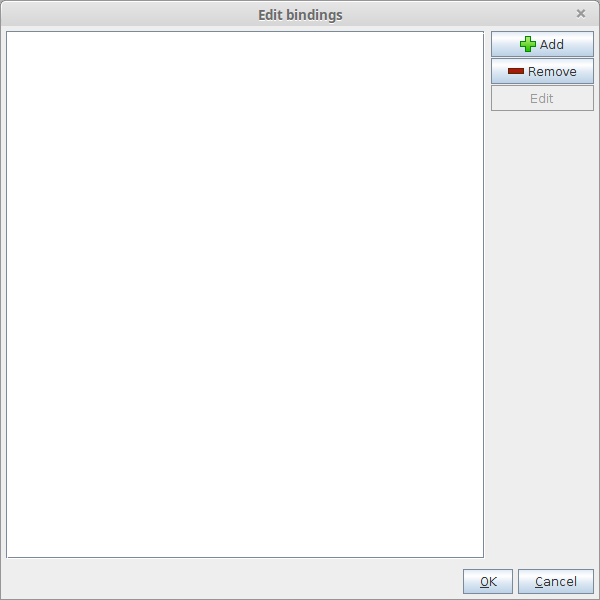
\includegraphics[width=7.0cm]{images/AnnotationEditBindingsDialog.png}
  \caption{Edit bindings dialog.}
  \label{AnnotationEditBindingsDialog}
\end{figure}

When editing a binding there are various options for customizing the output
from the binding.

The output from a binding is made up of a header and \textit{true} or
\textit{false} along with a timestamp:

\begin{verbatim}
Timestamp,Meta-Binding1,Meta-Binding2
00:00:00.000,false,false
00:00:01.000,false,true
\end{verbatim}

In this case the name of the binding shows up as \textit{Binding1} and
\textit{Binding2}. Figure \ref{add_binding} shows the dialog for editing a
binding.

\begin{figure}[htb]
  \centering
  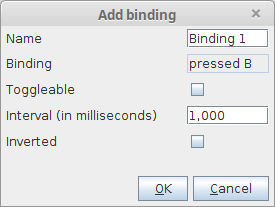
\includegraphics[width=4.0cm]{images/add_binding.png}
  \caption{Dialog for editing a binding.}
  \label{add_binding}
\end{figure}

In the following, an description of what each of the binding parameters is
used for:
\begin{tight_itemize}
  \item \textbf{Name} -- This is what gets output as the header of the
  annotation file when it is exported
  \item \textbf{Binding} -- The key for this binding. It is entered by
  selecting the text box and then pressing the desired key or key combination
  -- i.e. \texttt{ctrl + B} or just \texttt{B}
  \item \textbf{Toggleable} -- If this is checked then the binding always
  outputs a value, usually \textit{false}, and when it is toggled switches
  that output to \textit{true}.
  \item \textbf{Interval} -- Only relevant for toggleable bindings. This is
  the interval at which the values will be output. By default it is 1,000
  milliseconds (= 1 second) but it can be changed to any number. Intervals
  below 1 second tend to become less accurate, so if set at 10 ms it might
  output a value between 1 - 20 ms rather than 10 depending on CPU load and
  scheduling. It is recommended to use times of a second or above.
  \item \textbf{Inverted} -- This allows you to invert the values output
  by the binding. Usually a binding outputs \textit{true} when pressed or, in the
  case of toggleable bindings, toggled on. This will invert that so when
  it is pressed it will output \textit{false} and in the case of a toggleable it
  will output a value of \textit{true} when it is toggled off and \textit{false} when toggled on.
\end{tight_itemize}


%%%%%%%%%%%%%%%%%%%%%%%%%%%%%%%%%%%
\chapter{Data}
\section{.trail format}
The \textit{.trail} format is a simple text format. In its essence it is
spreadsheet-like format with a header and a body.

The \textit{header} contains the meta-data for the trail. Most importantly,
the width and the height of the trail. The format is in Java Properties format,
each line prefixed with ``\# ''. Each stored value also defines in a separate
property what data type it is (N = numeric, S = string, B = boolean).

It is possible to store an optional background image in the header. The image
data is stored as RGBA signed bytes, row-by-row. In order to produce smaller
files, the data is compressed using gzip\cite{gzip}. The compressed bytes are
then stored in a upper-case hexadecimal notation, with a maximum of 1000 bytes
per line. The background data lines are prefixed with ``\% ''.

The \textit{body} consists of four columns: timestamp (with milli-seconds), X position,
Y position, meta-data for that step. The meta-data column is a blank-separated list of
key-value pairs (``key=value"").

Here is an example file, without a background:

\begin{verbatim}
# #Tue Jul 28 09:24:20 NZST 2015
# Trail.Height\tDataType=N
# Trail.Width\tDataType=N
# Trail.Height=720.0
# Parent\ ID=-1
# Trail.Width=1280.0
Timestamp,X,Y,Meta-data
"00:00:00.127",424,292,""
"00:00:00.224",423,285,""
"00:00:00.304",423,277,""
\end{verbatim}


%%%%%%%%%%%%%%%%%%%%%%%%%%%%%%%%%%%
% Copyright (c) 2009-2012 by the University of Waikato, Hamilton, NZ. 
% This work is made available under the terms of the 
% Creative Commons Attribution-ShareAlike 4.0 license,
% http://creativecommons.org/licenses/by-sa/4.0/.
%
% Version: $Revision$

\begin{thebibliography}{999}
	% to make the bibliography appear in the TOC
	\addcontentsline{toc}{chapter}{Bibliography}

    % references
	\bibitem{adams}
		\textit{ADAMS} -- Advanced Data mining and Machine learning System \\
		\url{https://adams.cms.waikato.ac.nz/}{}
		
	\bibitem{heatmap}
		\textit{Heat map} -- WikiPedia article \\
		\url{http://en.wikipedia.org/wiki/Heat_map}{}

\end{thebibliography}


\end{document}
